\ifpdf
\graphicspath{{2_chronisch_obstruktive_lungenerkrankung/figures/PNG/}{2_chronisch_obstruktive_lungenerkrankung/figures/PDF/}{2_chronisch_obstruktive_lungenerkrankung/figures/}}
\else
\graphicspath{{2_chronisch_obstruktive_lungenerkrankung/figures/EPS/}{2_chronisch_obstruktive_lungenerkrankung/figures/}}
\fi

\chapter{Chronisch obstruktive Lungenerkrankung (COPD)}
\label{chapter:copd}

Die Chronisch obstruktive Lungenerkrankung, auf englisch Chronic Obstructive Pulmonary Disease (COPD) genannt, ist trotz ihrer starken Verbreitung noch vielen Menschen nicht bekannt.
Bei der COPD handelt es sich um eine chronische Lungenkrankheit mit progredienter Atemwegsverengung; sie gilt als die häufigste Erkrankung der Atmungsorgane (Darstellung der Atmungsorgane siehe Abbildung \ref{fig:atemsystem}). 


\begin{figure}
 \centering
  \includegraphics[width=1.0\textwidth]{atemsystem}
  \caption{Aufbau des Atmungssystems bis in die kleinsten Lungenstrukturen, die Alveolen. Eine Abbildung des Zwerchfells findet sich in Kapitel \ref{chapter:musiktherapeutische_stimmarbeit} (entnommen aus \cite[178]{schoppmeyer2012})}
  \label{fig:atemsystem}
\end{figure}

COPD ist ein Sammelbegriff für die chronisch obstruktive Bronchitis und das Lungenemphysem, welche entweder einzeln oder gemeinsam auftreten \autocite[vgl.][153]{lorenz2009}. Die COPD resultiert aus einer langfristigen Entzündung der Atemwege, welche durch ständige Belastung mit Zigarettenrauch, aber auch Umweltfaktoren, Staubpartikeln und giftigen Dämpfen entsteht. Ätiologisch wird davon ausgegangen, dass 80-90\% der COPD-Patienten die Erkrankung aufgrund von Nikotinabusus entwickelt haben; das sind in etwa 15\% der Zigarettenraucher\autocite[vgl.][154]{lorenz2009}. 

Als ein wichtiges Diagnosemerkmal gilt die Atemnot (Dispnoe), welche aus der Obstruktion der Bronchien resultiert (siehe Abbildung \ref{fig:copd_emphysem}). Diese wird durch drei Faktoren ausgelöst: 

\begin{enumerate}
\item Verkrampfung der Bronchialmuskulatur (Bronchospasmus)
\item Anschwellen der Schleimhaut in den Bronchien (Ödem)
\item Krankhaft erhöhte Schleimproduktion (Hyperkrinie) aufgrund einer dauerhaften Entzündung der Atemwege (chronische Bronchitis)
\end{enumerate}

Aufgrund der Bewegungseinschränkung durch die Hyperkrenie werden die Zilien - kleine Flimmerhärchen in den Bronchien - immer mehr daran gehindert, Schadstoffe aus der Lunge hinaus zu befördern. Dieser Prozess führt über einen längeren Zeitraum zur Zerstörung der Flimmerhärchen und somit zu einem größeren Exazerbationsrisiko (siehe unten).
Die Luftnot tritt im Anfangsstadium nur unter Belastung auf, später auch im Ruhezustand \autocite[vgl.][6f.]{lorenz2009}. Die allgemeine Symptomatik umfasst morgendlichen Kopfschmerz, Gewichtsverlust, welcher auf verstärkte Atemarbeit und systemische Entzündungsreaktionen zurückzuführen ist, zunehmenden Leistungsabfall, Einflussstauung, Ödeme der unteren Extremitäten und weiter abnehmende Belastbarkeit aufgrund des s.g. Cor pulmonale (Lungenherz, s. weiter unten).
Eine chronisch obstruktive Lungenerkrankung liegt laut WHO-Definition dann vor, wenn sowohl Husten und Auswurf über wenigstens als 3 Monate in mindestens 2 aufeinander folgenden Jahren bestehen und somit als chronisch anzusehen sind, als auch andere Krankheiten wie z.B. Bronchiektasen, Staubbelastung, cystische Fibrose, Asthma, Fremdkörper u.a. im Vorfeld ausgeschlossen werden konnten \autocite[vgl.][71]{koehler2010}. 

\begin{figure}
 \centering
  \includegraphics[width=0.6\textwidth]{copd_emphysem}
  \caption{Die Abbildung zeigt die typischen pneumologischen Veränderungen bei COPD und Lungenemphysem. Oben: Querschnitt eines gesunden (links) und eines entzündeten Bronchus. Unten: Die rechte Darstellung der Alveolen zeigt die krankhaft veränderte Struktur der Alveolarwände bei einem Lungenemphysem \cite[vgl.][16]{lingemann2014})}
  \label{fig:copd_emphysem}
\end{figure}

Das Lungenemphysem ist das Resultat länger andauernder Entzündungsreaktionen auf o.g. mögliche externe Partikel. Durch entzündliche Prozesse werden die Zellwände in den Alveolen (Lungenbläschen, siehe Abbildung \ref{fig:copd_emphysem}) zerstört. Hierfür sind Proteasen zuständig, die beim Eindringen von schädlichen Stoffen in die Lunge durch das Immunsystem freigesetzt werden. So genannte Antiproteasen können jedoch vor der Zerstörung der Alveolarwände schützen. Diese werden für normal körpereigen produziert; hierzu gehört u.a. das Alpha-1-Antitrypsin. Einige Patienten leiden jedoch unter einem genetische bedingen Alpha-1-Antrypsinmangel, wodurch ein erhöhtes Risiko für die Ausbildung eines Lungenemphysems besteht.
Das bedeutet, dass sich mit weiterbestehender Entzündung die Anzahl der für den Sauerstoff-Kohlendioxid-Austausch notwendigen Alveolen verringert und sich die Lufträume in der Lunge vergrößern. Dadurch wird nach und nach die Lungenelastizität eingeschränkt, was eine Überdehnung der Lunge (Hyperinflation) mit Minderdurchblutung und einem irreversiblen Schwund an Lungengewebe als auch eine Einschränkung der Atemfunktion nach sich zieht. Dies geschieht jedoch nicht nur durch die degenerativen Prozesse in einem Lungenlappen, sondern auch durch funktionelle Beeinträchtigung anderer umliegender, gesunder Lungenlappen aufgrund der partiellen Überblähung. Auch andere Organe können möglicherweise beschädigt werden. Denn bei Nichtbehandlung des Emphysems kommt es zu einer erhöhten Pumpleistung des Herzmuskels und so über längere Zeit zu einer Schädigung desselben, da dieser nun mehr Blut transportieren muss, um die Organe ausreichend mit Sauerstoff zu versorgen. So ist vor allem das Endstadium der COPD gekennzeichnet durch das Auftreten des so genannten Cor Pulmonare, dem Lungenherz. Hiermit ist die Rechtsherz-Insuffizienz gemeint, bei welcher die rechte Herzkammer aufgrund des Blutstaus durch den langsameren Sauerstoff-Kohlendioxid-Austausch in den Lungen immer größer wird und an Leistungskraft verliert \autocite[vgl.][e10]{vogelmeier2007}.

Bei Fortschreiten der COPD kommt es immer wieder zu Exazerbationen, das heißt zu akuten Verschlechterungen der alltäglichen Krankheitssymptome, was zu Symptomen wie Atemnot, Husten, vermehrter Sputummenge oder Fieber führen kann. Sie resultieren zu 60-70\% aus einer Infektion der Lunge oder nichtinfektiösen Ursachen wie akuter Luftverschmutzung oder Verschlechterung von Begleiterkrankungen und sollten daher zeitnah behandelt werden.

Das Auftreten der COPD nimmt mit dem Alter zu, dabei kommt es ab dem 50. Lebensjahr zu einem rapiden Anstieg der Prävalenz. Im siebten Dezennium ist die Spitze des Auftretens mit etwa 10\% bei Männern und ca. 5\% bei Frauen erreicht\autocite[vgl.][153]{lorenz2009}. Nach Köhler/Schönhofer/Voshaar (2010) sei Vorsicht geboten bei dem Einbezug von Statistiken in diesem Bereich, da die verfügbaren Daten zur Prävalenz der COPD sehr von dem untersuchten Kollektiv bzw. den Altersgruppen abhängen (vgl. ebd., 72). Insgesamt gehen sie jedoch von folgenden Zahlen aus: Etwa 10\% der deutschen Bürger ab dem 40. Lebensjahr seien davon betroffen, wobei ca. 10\% dieser Patientenkohorte einen höheren Schweregrad (siehe Tabelle \ref{tab:copd_schweregrade})  aufweisen. Es wird davon ausgegangen, dass den Hausärzten nur etwa bei der Hälfte der Patienten die Erkrankung bekannt ist.
In Bezug auf die Mortalität gilt bei ca. 3,5\% aller Todesfälle COPD als die Haupttodesursache. Allerdings ist sie bei ca. 4,5\% der Todesfälle mitverursachend. Es wird davon ausgegangen, dass COPD auf der Liste der häufigsten Todesursachen in den nächsten 6 Jahren weltweit von dem 4. auf den 3. Platz aufsteigen wird.
Laut der COPD-Leitlinie besteht eine hohe sozioökonomische Belastung durch die steigende Zahl an COPD-Fällen. In der Hochrechnung von Krankenhausstatistiken seit 1996 wurden für obstruktive Atemwegserkrankungen 2,7 Mio. Krankenhaustage erfasst. Einen Großteil macht hierbei die Behandlung chronischer Bronchitis und ihrer Folgen aus. Auch die von der AOK hochgerechneten jährlichen Krankheitstage in Höhe von 25 Mio. aufgrund der chronischen Bronchitis sind immens. Sie entsprechen volkswirtschaftlichen Gesamtkosten von etwa 5,93 Mrd. Euro jährlich \autocite[vgl.][e4]{vogelmeier2007}.

Um das Krankheitsbild, Diagnostik und Therapie weltweit zu vereinheitlichen, wurde der o.g. englische Begriff eingeführt. Eine globale Initiatve, welche 2001 von der Weltgesundheitsorganisation (WHO) und den National Institutes of Health (NIH) gegründet wurde, hat zusätzlich dazu beigetragen, dass weltweit eine einheitliche Leitlinie, die s.g. GOLD-Leitlinie, zum Tragen kommt. Die Erkrankung wird hiernach in vier Schweregrade eingeteilt, die sich an dem gemessenen Ausatemvolumen orientieren. Einige Autoren, darunter Köhler/Schönhofer/Voshaar \autocite[vgl.][75]{koehler2010}, bewerten diese Leitlinie jedoch als einen Rückschritt, da diese das Krankheitsbild in Bezug auf seine Pathophysiologie zu sehr vereinfache.

Diese Einteilung wird jedoch in der Praxis nach wie vor vorgenommen, weshalb sie an dieser Stelle dargestellt werden soll.

In den GOLD-Leitlinien wird zwischen 4 Stadien unterschieden. Für die Einteilung kommen 2 Werte der Lungenfunktionsprüfung (siehe Kapitel \ref{diagnostik}) zum Tragen. Der erste Wert, das forcierte exspiratorische Volumen ($FEV_{1}$) gibt Auskunft darüber, wieviel Luft eine Person innerhalb einer Minute forciert ausatmen kann. Für eine Einstufung wird der $FEV_{1}$-Wert eines Patienten mit Soll- bzw. Normalwerten verglichen, welche wiederum abhängig von Geschlecht, Alter und Körpergröße des Patienten sind. Dieser Wert gilt in der Regel als Indikator für die Schwere der Erkrankung. In diesem Zusammenhang ist auch das Verhältnis zwischen der inspiratorischen Vitalkapazität (Einatemvolumen) und dem $FEV_{1}$ für die Diagnosestellung wichtig (siehe Tabelle \ref{tab:copd_schweregrade}). Bei der leichtgradigen COPD (Schweregrad I) besteht die Atemwegsobstruktion ohne eine signifikante $FEV_{1}$-Verminderung. Patienten in diesem Stadium berichten über chronischen Husten und Auswurf, bemerken jedoch meist noch keine Einschränkung ihrer Lungenfunktion. Beim Schweregrad II besteht neben der Atemwegsobstruktion bereits eine geringe $FEV_{1}$- Verminderung und die kranksheitsspezifischen Symptome, insbesondere Dyspnoe unter Belastung, nehmen zu. Die schwere COPD (Schweregrad III) ist charakterisiert durch eine höhergradige $FEV_{1}$-Verminderung, das heißt $FEV_{1}$-Werten zwischen 30\% und 50\% des Soll. Es besteht jedoch nur eine geringe oder keine Korrelation zwischen dem Ausmaß der Dyspnoe und dem Schweregrad der Lungenfunktionseinschränkung. Für den Schweregrad IV gilt ein $FEV_{1}$-Wert von $\leq$ 30\% Soll als ausschlaggebend. Bei einer gleichzeitigen respiratorischen Insuffizienz darf für die Einteilung in den Schweregrad IV der $FEV_{1}$-Wert $<$50\% soll betragen \autocite[vgl.][e8]{vogelmeier2007}.

\begin{table}
\centering
\begin{tabular}{lp{10cm}}
	\textbf{Schweregrad} & \textbf{Kriterien} \\
	\hline \hline
	I (leicht) & $FEV_{1} \ge 80\% Soll, FEV_{1}/VC < 70\%$ \newline mit/ohne Symptomatik (Husten, Auswurf) \\
	\hline
	II (mittel) & $50\% Soll \le FEV_{1} < 80\% Soll, FEV_{1}/VC < 70\%$ \newline mit chronischen Symptomen/ohne chronische Symptome (Husten, Auswurf, Dyspnoe) \\
	\hline
	III (schwer) & $30\% Soll < FEV_{1} < 50\% Soll, FEV_{1}/VC < 70\%$ \newline mit chronischen Symptomen/ohne chronische Symptome (Husten, Auswurf, Dyspnoe) \\
	\hline
	IV (sehr schwer) & $FEV_{1} \le 30\% Soll, FEV_{1}/VC < 70\%$ oder \newline $FEV_{1} < 50\% Soll$ plus chronische respiratorische Insuffizienz \\
	\hline
\end{tabular}
\caption{Schweregradeinteilung der COPD, aus \autocite[e9]{vogelmeier2007}}
\label{tab:copd_schweregrade}
\end{table}

Eine neuere, multidimensionale Schweregradbeurteilung stellt der s.g. BODE-Index dar (siehe Anhang). Dieser bezieht in seine Bewertung den Body-Mass-Index (B), die $FEV_{1}$-Einschränkung (O, Obstruction), das Dyspnoeempfinden (D) und die Belastbarkeit (E, exercise capacity) mit ein. Dabei wird eine Aussage über das Dyspnoeempfinden mittels des leicht abgeänderten Medical Research Council (MRC)-Scores vorgenommen, der folgendermaßen eingeteilt ist: "`0 = keine Atemnot, 1 = Atemnot bei schwerer Belastung, 2 = Atemnot bei leichter Belastung, 3 = zu atemlos, das Haus zu verlassen und atemlos beim An- und Ausziehen"' \autocite[186f.]{welte2007}. Die Belastbarkeit wird durch den 6-Minuten-Gehtest gemessen, welcher sich nach der zurückgelegten Strecke in Metern orientiert.


\section{Diagnostik} % section headings are printed smaller than chapter names
\label{diagnostik}
Um eine Verdachtsdiagnose stellen zu können, wird zu Beginn eine umfangreiche \emph{Anamnese} durchgeführt. Diese umfasst folgende, auf COPD verweisende Kriterien: Alter, Familienanamnese, Husten, Auswurf, Atemnot unter Belastung, Rauchgewohnheit und/oder inhalative Belastung am Arbeitsplatz, Anzahl der Exazerbationen pro Jahr, gegenwärtige Medikation, Beeinträchtigung im Alltag, Sozialanamnese, Störungen der Atmung im Schlaf, mögliche Komorbiditäten (s. weiter unten) und Gewichtsverlust. 

Folgende \emph{körperliche Untersuchungsbefunde} geben ebenfalls Hinweis auf eine mögliche COPD, wobei bei einer leichtgradigen Ausprägung der Erkrankung diese Befunde unauffällig sein können: bei einer mittelgradigen COPD deuten verlängertes Exspirium, Giemen, Pfeifen und Brummen auf eine Obstruktion der Atemwege, ein tief stehendes, wenig verschiebbares Zwerchfell und hypersonorer Klopfschall auf eine Lungenüberblähung hin. 

Einen sehr wichtigen Teil der Diagnostik stellen \emph{Lungenfunktionstestungen} dar, weil sie einerseits für die Einteilung der Schweregrade gebraucht werden. Andererseits können sie Aussagen über eine nicht vollständig reversible Atemwegsobstruktion durch Nicht-Ansprechen auf die Gabe von Bronchodilatatoren und/oder Glukokortikoiden (siehe auch Kapitel \ref{medikamentoese_therapien}) treffen, was ein klares Indiz für eine ausgebildete COPD darstellt. Dieser Reversibilitätstest ist insbesondere für die Differenzialdiagnose zwischen Asthma und COPD entscheidend. 

Die gängigsten Lungenfunktionstests sind die Spirometrie und die Ganzkörperplethysmographie. Bei der Spirometrie wird durch Ein- und Ausatmen in ein hierfür spezialisiertes Gerät gemessen, wie viel Luft durch die Lunge aufgenommen und wie schnell diese gefüllt und wieder geleert werden kann. Hier wird sowohl der oben mehrmals erwähnte $FEV_{1}$-Wert als auch die forcierte Vitalkapazität (FVC) ermittelt. Je niedriger der $FEV_{1}$-Wert ausfällt, desto schlechter ist die Lungenkapazität. Bei der Ganzkörper-, auch Bodyplethysmographie genannt, wird hingegen gemessen, wieviel Luft in der Lunge nach der maximalen Ausatmung in der Lunge verbleibt. Das Ergebnis bildet sich in der s.g. funktionellen Residualkapazität (FRC) ab \autocite[vgl.][e6f.]{vogelmeier2007}. Bei einem Lungenemphysem wird das Residualvolumen größer sein als bei vergleichbaren gesunden Menschen. 

Ein weiteres Verfahren ist die \emph{arterielle Blutgasanalyse}, welche zur Abklärung einer Gasaustauschstörung, auch respiratorische (Partial-)Insuffizienz genannt, sowie zur therapeutischen Abschätzung der Indikation für eine Sauerstofftherapie dient \autocite[190]{welte2007}.

Wie bereits oben erwähnt, gehören auch \emph{Belastungstests} zur COPD-Diagnostik. Diese sollen Aufschluss über die verschiedenen Ursachen der Belastungsdyspnoe und die Therapieeffekte von Medikamenten und Orientierung zur Erstellung eines individuell angepassten Trainingsprogramms im ambulanten als auch rehabilitativen Bereich geben \autocite[vgl.][e7]{vogelmeier2007}. 

\emph{Bildgebende Verfahren} wie z.B. Röntgenaufnahmen und Computertomografie (High Resolution, HR-CT) der Thoraxorgane sind für die Diagnostizierung eines Lungenemphysems sowie für die Differenzialdiagnostik (insbesondere zum Ausschluss eines Bronchialkarzinoms oder kardialer Erkrankungen) von großer Bedeutung. \autocite[191]{welte2007}.

Zudem werden aufgrund des Zusammenhangs der COPD mit kardialer Belastung auch Echokardiographie und Elektrokardiogramm eingesetzt.

Da es sich bei der COPD um eine progrediente Erkrankung mit fließenden Übergängen handelt, bedarf es einer aufmerksamen und regelmäßigen fachärztlichen Versorgung, welche die Funktionsparameter und klinischen Symptome mindestens einmal jährlich bzw. bei Verschlechterung der Krankheitssymptome überprüft \autocite[vgl.][e8ff.]{vogelmeier2007}.

Bei Interesse können die zuvor beschriebenen Inhalte der Diagnostik bei COPD in einer Tabelle in Form eines nachvollziehbaren Algorithmus im Anhang nachvollzogen werden.

\section{Behandlungsmethoden}
\label{behandlungsmethoden}
Die Behandlung bei COPD schließt neben Raucherentwöhnung, medikamentöser Therapie, Patientenschulung, Physiotherapie, körperlichem Training, Ernährungsberatung sowie apparativer Therapiemöglichkeiten bei schwererem Lungenemphysem auch chirurgische Maßnahmen ein; traditionell läge der Schwerpunkt jedoch auf der medikamentösen Therapie, so Lang \autocite[vgl.][287]{lang2007}. Die Therapieziele umfassen in erster Linie die Rückbildung von Dyspnoe, Husten und Auswurf, Verbesserung der Belastbarkeit, längere Lebenserwartung und die Senkung der Exazerbationsfrequenz. Atemphysiologisch wird sowohl ein Anstieg des $FEV_{1}$- und $p_{2}O_{2}$ -Wertes angestrebt als auch ein Abfall von Atemwegswiderstand, thorakalem Gasvolumen, Residualvolumen und $paCO_{2}$ \autocite[vgl.][158]{lorenz2009}
Die o.g. verschiedenen Behandlungszweige werden in den beiden folgenden Kapiteln kurz dargestellt.

\subsection{Medikamentoese Therapien}
\label{medikamentoese_therapien}
Aufgrund häufiger Komorbiditäten bei COPD und mehreren Symptomen dieser komplexen Erkrankung bedarf es einer individuell angepassten pharmazeutischen Behandlung der Patienten, welche pneumologisch gut abgeklärt sein sollte. Die medikamentöse Behandlung hat keinen Einfluss auf den progredienten Verlauf der Erkrankung. Sie kann jedoch zur Linderung der Beschwerden, einer Verbesserung der körperlichen Leistungsfähigkeit, der Lebensqualität und zur Reduktion von Exazerbationen beitragen \autocite[vgl.][249]{gillissen2007}. In der Fachliteratur wird immer wieder darauf verwiesen, dass die Pharmakotherapie bei Rauchern mit COPD immer flankiert sein sollte durch Raucherentwöhnungsprogramme (siehe Kapitel \ref{nicht-medikamentoese_therapien}), um die Langzeitprognose zu verbessern. Die psychosoziale Begleitung in Verbindung mit einer Nikotinersatztherapie und einer angemessenen Nachsorge sowie Rückfallintervention gilt als besonders erfolgsversprechend. Darüber hinaus kann die Vergabe des Antidepressivums Bupropion zusätzlich die Entwöhnungsrate steigern \autocite[vgl.][e12]{vogelmeier2007}.

Bei der Pharmakotherapie bildet die Gruppe der Bronchodilatatoren ($\beta$2- Sympathomimetika, Anticholinergika, Theophyllin) die Basismedikation, welche i.d.R. in inhalativer Form verabreicht wird.
Medikamente dieser Wirkstoffgruppe entspannen die Muskeln in den verengten Atemwegen und verbessern so die Luftzufuhr, jedoch setzen sie an unterschiedlichen Stellen an.

Eine wichtige Wirkstoffgruppe, vorallem für die Behandlung von Patienten mit schwerer COPD ab dem Schweregrad 3 und/ oder mit rezidivierenden Exazerbationen, stellen inhalative Kortikosteroide [ICS] dar. Es handelt sich hierbei um entzündungshemmende Medikamente, die die Entzündungsreaktion in den Lungen und die Schwellung der Bronchien vermindern. In der Regel wird jedoch eine Kombinationstherapie mit ICS und langwirksamen $\beta$2-Sympthomimetika eingesetzt, da diese sich in Studien als besonders wirksam herausstellte. Die systemische Kortisontherapie ist im Einzelfall bei akuten Exazerbationen kurzfristig indiziert, wird jedoch kaum als Dauerbehandlung eingesetzt \autocite[vgl.][249f., 253]{gillissen2007}.

\subsection{Nicht-medikamentöse Therapien}
\label{nicht-medikamentoese_therapien}
Als vorrangiges Ziel der Prävention gilt die Reduktion inhalativer Schadstoffe im näheren Umfeld des Patienten. Hierbei steht der Verzicht auf Nikotinkonsum an oberster Stelle, weshalb ein wichtiger Bereich der nicht-medikamentösen Therapie \emph{Raucherentwöhnungsprogramme} darstellen. Durch einen Rauchstopp kann ein schnelleres Fortschreiten der Erkrankung verhindert und eine bessere Voraussetzung für eine erfolgreiche Behandlung geschaffen werden. Daneben kann die Prävalenz von Exazerbationen und das Risiko für Komorbiditäten gesenkt werden.

In der \emph{physiotherapeutischen Atemtherapie} erlernen die Patienten einen bewussten Umgang mit ihrer Atmung mithilfe von atemerleichternden Stellungen sowie Atemtechniken. Eine sehr wichtige Atemtechnik zur Verringerung der akuten Atemnot stellt die „Lippenbremse“ dar. Hierbei wird die Luft durch die besonders enge Stellung der Lippen sehr dosiert ausgeatmet und wirkt durch den aufgebauten Druck bronchienerweiternd. Diese Atemtechnik wird möglichst mit atemerleichternden Stellungen kombiniert (Kutschersitz, „Hängebauchschwein“, Torwartstellung, Wandstütze u.a.), welche den Thorax vom Gewicht des Schultergürtels entlasten und zudem das „Längenspannungsverhältnis der Atemhilfsmuskulatur und des Zwerchfells“ verbessern \autocite[vgl.][291]{lang2007}. Einen weiteren wichtigen Bereich der Atemtherapie bildet die Koppelung von Atmung und Bewegung. Hierbei wird die eigene Atmung von körperlichen Bewegungen, wie z.B. im Liegen beim Einatmen den Arm über die Seite nach oben und beim Ausatmen wieder zurückführen, begleitet. Hierdurch werden Belastungssituationen in einem geschützten Rahmen simuliert und erprobt.

Besonders wichtig für die Prävention von Exazerbationen ist die so genannten Sekretdrainage, ein Bereich der \emph{physikalischen Therapie}. Hier gilt es, durch bestimmte Körperdehnlagerungen und Handgriffe, welche die Atembewegung unterstützen oder einen erhöhten Widerstand erzeugen sowie durch Vibrationen das Sekret zu mobilisieren und so das Abhusten zu erleichtern. Durch die Dehnlagerungen wird das Zwerchfell aktiviert, die Atembewegung vertieft und die Rippenbeweglichkeit verbessert.

Des Weiteren führen solche Dehnübungen zur besseren Durchlüftung und Durchblutung der Lunge. 
Darüber hinaus kommt auch dem körperlichen Training eine wichtige Rolle in der Langzeittherapie zu, da hierdurch gerade bei Patienten ab Schweregrad II die Lebensqualität und Belastbarkeit signifikant gesteigert sowie die Exazerbationsrate gesenkt werden kann. Wichtig ist dabei, dass ein während einer Rehamaßnahme individuell erstellter Trainingsplan auch Zuhause weiter geführt wird. Besonders eignen sich für diese Patientengruppe Sportarten, welche die Ausdauerleistungsfähigkeit trainieren. Hierzu gehören Joggen, Schwimmen, Fahrradfahren, Inline-Skating und (Nordic-)Walking sowie im Winter Langlauf. Dabei sollten Outdoor-Aktivitäten jedoch möglichst in der Natur durchgeführt werden, da in den Städten und Ortschaften meist die Feinstaubbelastung durch Autoabgase, Fabriken etc. erhöht ist. In größeren Städten werden zudem Lungensportgruppen angeboten, was m.E. gerade bei COPD-Patienten im Hinblick auf mögliche Komorbiditäten (siehe Kapitel \ref{komorbiditaeten}) sehr sinnvoll erscheint. Bei einigen Patienten kann wegen ausgeprägter muskulärer Dekonditionierung vorerst Krafttraining angezeigt sein \autocite[vgl.][291f]{lang2007}.

Einen weiteren Bestandteil der nicht-medikamentösen Therapie bildet die \emph{Ergotherapie}. Hier können Fertigkeiten für den Alltag und die Teilhabe an der Gesellschaft geschult und erweitert werden.

Auch \emph{Patientenschulungen} sind wesentlich für das Management der COPD. 
In strukturierten Schulungsprogrammen werden Patienten Grundkenntnisse über Anatomie und Krankheitsbild und Behandlungsmöglichkeiten vermittelt. Darüber hinaus dienen sie als Verhaltenstraining, da hier auch konkrete Handlungsanweisungen in Bezug auf präventive Faktoren wie Raucherentwöhnung und Infektionsprophylaxe, Verbesserung des Krisenmanagements inklusive der Erarbeitung eines Krisenplanes als auch die richtige Handhabung der Inhalatoren und bestimmte Atemtechniken (s. oben) vermittelt werden.

\emph{Entspannungsverfahren} bewirken vielfache positive physiologische Veränderungen und sind bei COPD besonders angezeigt. Es werden in erster Linie autogenes Training oder progressive Muskelentspannung nach Jacobson sowie Qi Gong empfohlen.

Gerade bei sehr leistungseingeschränkten Patienten bieten sich zur Unterstützung im Alltag \emph{Hilfsmittel} an. Darunter fallen u.a. Duschsitze und -halterungen, Hilfen beim Anziehen wie verlängerte Schuhanzieher und natürlich auch Rollatoren, die für die Mobilität vieler Patienten mit gleichzeitiger Atementlastung durch das nach vorn gebeugte Gehen sehr hilfreich sind.

In einigen Fällen ist bei chronischer Überlastung der Atemmuskulatur zur Atemmuskelermüdung eine \emph{Heimbeatmung} abzuwägen. Eine Indikation zur intermittierenden nichtinvasiven Beatmung Zuhause bei chronischer ventilatorischer Insuffizienz ist dann gegeben, "`wenn alle konservativen Behandlungsmöglichkeiten ausgeschöpft sind und der Patient weiterhin hyperkapnisch ist"' \autocite[e22]{vogelmeier2007}. Bei Patienten im Stadium IV, welche bereits unter einer chronischen Hypoxämie, das heißt mit einer Sauerstoff-Mangelversorgung, leiden, ist darüber hinaus eine \emph{Langzeitsauerstofftherapie} indiziert. Hierdurch können bei Anwendung über 16-24 Stunden/Tag die Prognose sowie weitere vorherrschende Symptome der COPD verbessert werden \autocite[vgl.][e22]{vogelmeier2007}

Die zuvor aufgeführten Bereiche der (nicht-)medikamentösen Therapie sind ebenfalls Bestandteil der \emph{pneumologischen Rehabilitation}, welche in den letzten Jahren aufgrund mittlerweile gesicherter positiver Effekte sehr an Wichtigkeit zugenommen haben. Als Hauptziele gelten die "`Linderung der physischen und psychischen Beeinträchtigung des Patienten, die Steigerung der Lebensqualität mit Wiederherstellung der bestmöglichen Leistungsfähigkeit sowie die Förderung der sozialen Reintegration"' \autocite[e21]{vogelmeier2007}. Die Durchführung findet entweder im ambulanten, teilstationären oder stationären Rahmen über mehrere Wochen (i.d.R. 3-6 Wochen) statt und beruht stets auf einem interdisziplinären und multimodalen Ansatz. Zu den o.g. Bereichen kommen noch soziale, sozialmedizinische und psychologische Diagnostik und Betreuung sowie Ernährungsberatung hinzu. 

Bei schwerem bis sehr schwerem Lungenemphysem können \emph{chirurgische Eingriffe} in manchen Fällen eine Behandlungsoption darstellen. Zu den momentan durchgeführten Verfahren gehören die s.g. Bullektomie (Entfernung von Lungenblasen), Lungenvolumenreduktion sowie als letzte Option die Lungentransplantation. Darüber hinaus wurden in den letzten Jahren weitere minimal invasive Techniken entwickelt, welche unter dem Begriff bronchoskopische Lungenvolumenreduktion zusammengefasst werden. Diese haben zum Vorteil, dass die Entfernung eines Lungenlappens nicht erforderlich ist \autocite[vgl.][e23]{vogelmeier2007}.

\section{Komorbiditäten}
\label{komorbiditaeten}
Das Thema "`Begleiterkrankungen bei COPD"' ist bereits zuvor an einigen Stellen angeklungen. Obgleich Leitlinien den Einfluss fachübergreifender Komorbiditäten oftmals außer Acht lassen, sind diese für die gesundheitsbezogene Lebensqualität laut König wichtiger als das $FEV_{1}$, demografische Faktoren oder Atemwegssymptome. Auch der Einfluss von Komorbiditäten auf die Mortalität stellt einen signifikanten Indikator dar \autocite[vgl.][395]{koenig2007}.
Daher soll diesem wichtigen Aspekt an dieser Stelle Rechnung getragen werden und anschließend auf körperliche und psychische Begleiterkrankungen näher eingegangen werden. Letzteres wird jedoch aufgrund der hohen Relevanz für das in dieser Arbeit entwickelte musiktherapeutische Konzept schwerpunktmäßig behandelt.


\subsection{Körperliche Komorbiditäten}
Wie bereits unter Kapitel \ref{einleitung} erwähnt, entwickeln viele COPD-Patienten im Krankheitsverlauf körperliche Begleiterkrankungen. Sehr häufig kommt es zu Herz-Kreislauf-Erkrankungen, die aus einem unzureichenden Gasaustausch resultieren. Die Herzinsuffizienz tritt so beispielsweise bei ca. 30\% der COPD-Patienten auf und für jeden 2. bestehe laut Stiefelhagen eine arterielle Hypertonie. 25\% der COPD-Betroffenen leiden zudem unter einer hämodynamisch wirksamen koronalen Herzerkrankung, was vermutlich dem Nikotinabusus geschuldet ist \autocite[vgl.][37]{stiefelhagen2013}.

Eine weitere häufige Komorbidität stellt Osteoporose dar. Stiefelhagen zufolge habe dies unterschiedliche Gründe: "`Immobilität, Alter, Gewichtsverlust, Steroid-Medikation, die COPD-typische systemische Entzündung und auch Nikotinabusus"' \autocite[37]{stiefelhagen2013}. An anderen Stellen wird diese Begleiterkrankung oftmals als Nebenwirkung der medikamentösen Behandlung hervorgehoben. 

Die gleichzeitige Prävalenz von COPD und Typ-2-Diabetes korreliert ebenfalls in vielen Fällen. Dies wird auf die systemische Inflammation als ein „pathogenetisches Bindeglied“ zurückgeführt, da sowohl die obstruktive Lungenerkrankung als auch der Diabetes mellitus Entzündungsprozesse beeinflussen.

Nicht zuletzt tritt im Zusammenhang mit der COPD auch immer wieder Lungenkrebs auf, welcher ebenfalls meist aus einem langjährigen Zigarettenkonsum resultiert \autocite[vgl.][38]{stiefelhagen2013}.


\subsection{Psychische Komorbiditäten}
\label{psychische_komorbiditaet}
Einen sehr wichtigen, vielfach nicht berücksichtigten Bereich bei einer COPD-Erkrankung stellen psychische Komorbiditäten dar.
Beinahe die Hälfte dieser Patientengruppe leidet zusätzlich zu ihrer körperlichen Erkrankung unter Angst- und Panikstörungen und/oder Depressionen; es wird zudem von einer hohen Dunkelziffer ausgegangen \autocite[vgl.][157]{fischer2007}.
Nach Steinkamp et. al kommen als Ursache für psychische Störungen bei COPD unterschiedliche Faktoren in Frage.
Diese umfassen: Nikotinabhängigkeit, eigenständige psychiatrische Krankheit, Hypoxämie, Hyperkapnie, Atemnot, Schlafstörungen, Einschränkung der Belastbarkeit und Mobilität und Vereinsamung \autocite[vgl.][157]{fischer2007}.
 
In wieweit jedoch diese Psychopathologien als Folge der COPD gesehen werden können oder relevante Koinzidenzen darstellen, ist noch ungeklärt. 

In den meisten Fällen bezieht man sich in der Literatur auf ein Krankheitsmodell, welches in der GOLD-Leitlinie aber auch in der Leitlinie der Atemwegsliga zu finden ist. Hierin wird von einem Teufelskreis (siehe Grafik  \ref{fig:copd_teufelskreis}), "`Circulus virtuosus"', ausgegangen, wonach die körperliche Leistungseinschränkung aufgrund vorherrschender Atemnot im Verlauf der Erkrankung zum Rückzug aus alltäglichen Abläufen und so immer mehr zur Immobilität und sozialen Isolation führt. 
Dadurch werden jedoch auch Angst und Depression immer weiter verstärkt. 

\begin{figure}
 \centering
  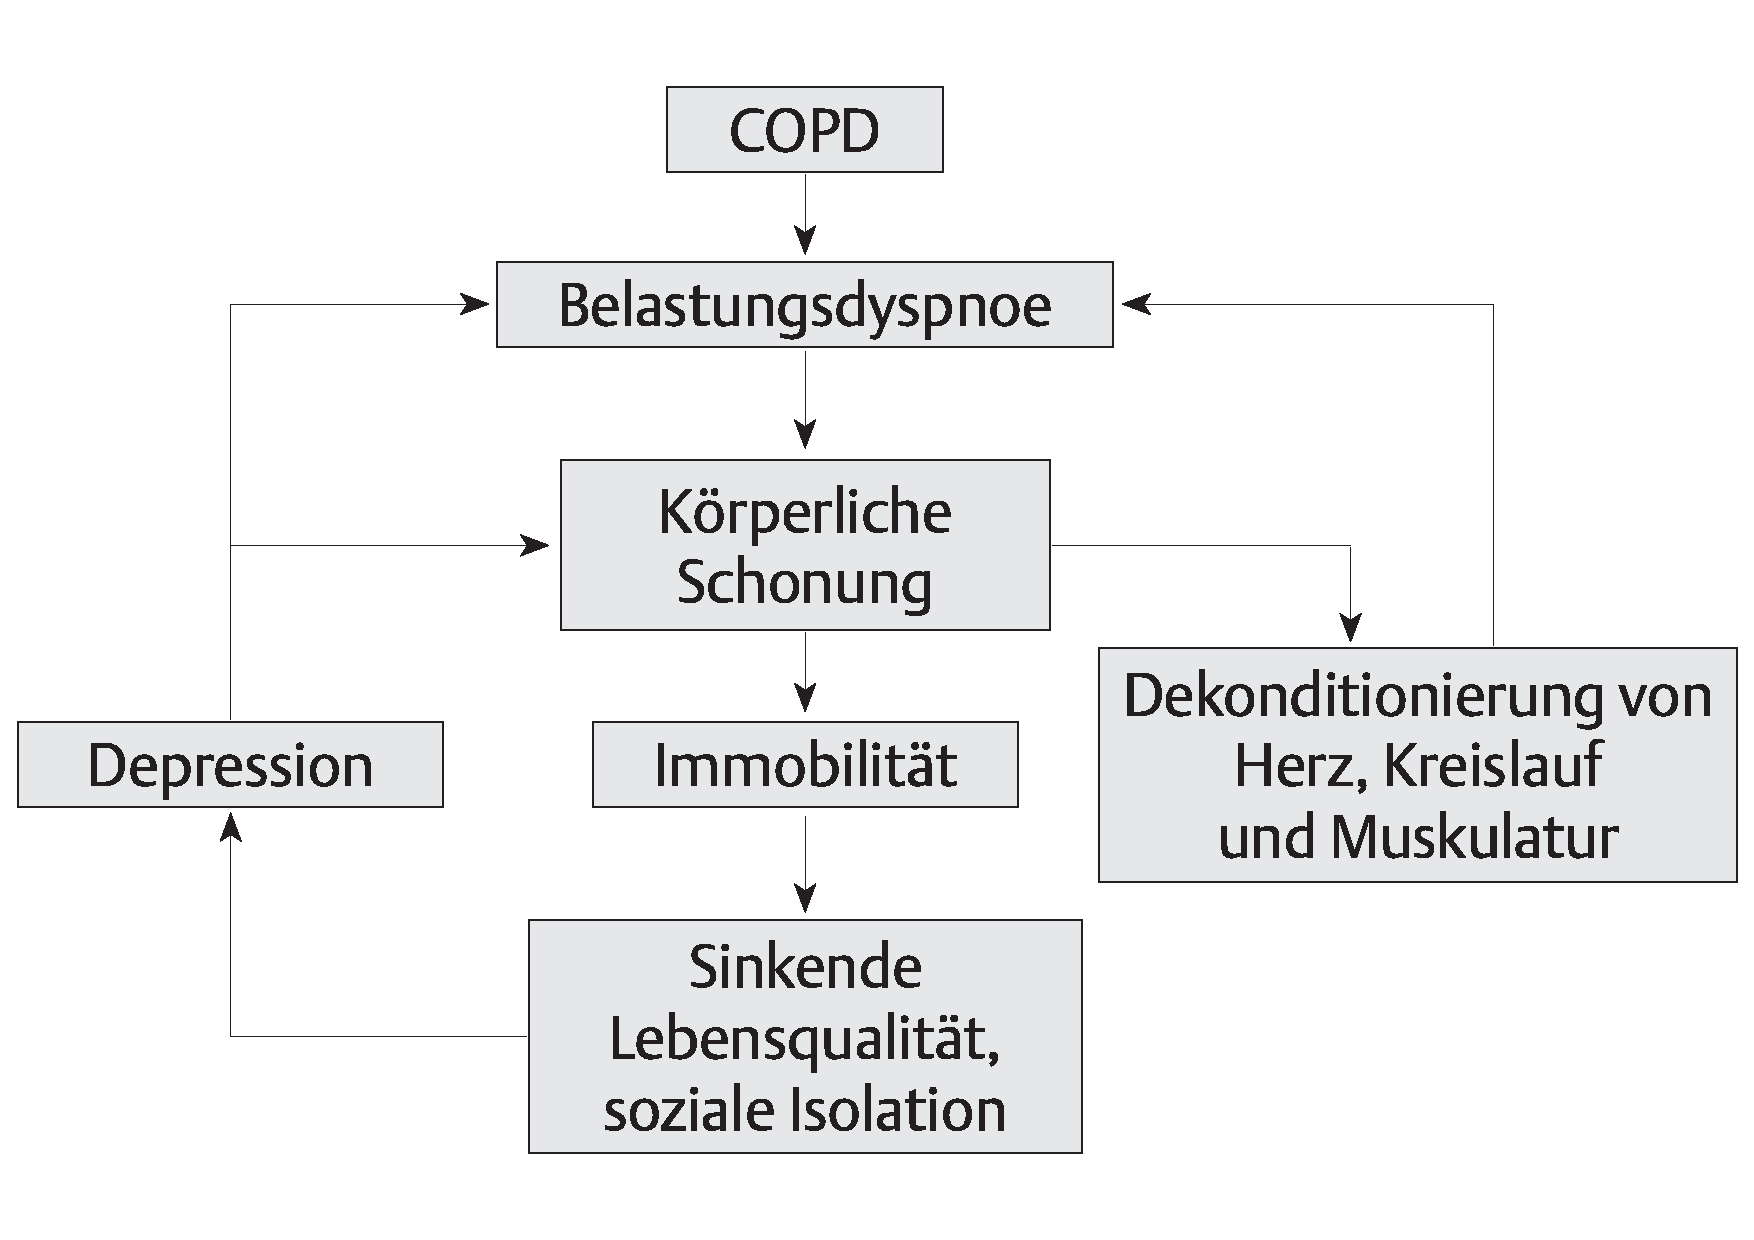
\includegraphics[width=0.6\textwidth]{teufelskreis}
  \caption{Circulus virtuosus, übernommen aus \cite[e19]{vogelmeier2007}}
  \label{fig:copd_teufelskreis}
\end{figure}

Die Angaben zur Prävalenz von Angst und Depression bei COPD variieren sehr. „Generalisierte Angststörungen werden in einer Häufigkeit von 2-16\%, Panikstörungen von 8-67\%, depressive Symptome und Depressionen zwischen 11 und 80\% sowie Angstsymptome in einem Bereich von 10-75\% angegeben“  \autocite[34]{kenn2011}.

An diesen Zahlen lässt sich erkennen, dass exakte Ergebnisse in Bezug auf die Prävalenz noch fehlen. Kenn und Kühl gehen davon aus, dass hierfür verschiedene methodische Diagnoseansätze verantwortlich sind. Generell erschwerte wohl neben den unterschiedlichen Erhebungsinstrumenten, wie Interviews und Fragebögen, auch die Heterogenität der untersuchten Patientenkohorte mit verschiedenen Schweregraden die Interpretation der Ergebnisse \autocite[vgl.][35]{kenn2011}.
Zudem geben die Studienergebnisse keine Auskunft darüber, in wieweit bei Patienten, die eine COPD aufgrund eines längeren Nikotinabusus entwickelt haben, bereits eine größere psychische Vulnerabilität und somit ein erhöhtes Risiko für die Ausbildung einer Depression oder Angst-/Panikstörung besteht. 

Ein evtl. wichtiges Konzept für den Krankheitsverlauf der COPD in seinen unterschiedlichen Facetten scheint die so genannten "`Fear Avoidance"' zu sein. Viele Patienten berichten von Angst vor auftretender Atemnot. Fear Avoidance- Konzept meint "`die Angst vor der Verstärkung eines Krankheitssymptoms bzw. Verschlechterung des Verlaufs und daraus folgende Aktivitätsvermeidung"' \autocite[111]{stenzel2013}. Dieses Konzept wurde jedoch bisher für COPD noch kaum diskutiert und erforscht. Eine neuere Studie zeigte jedoch, dass Fear Avoidance tatsächlich als Mediator des Zusammenhangs zwischen COPD-Status und Lebensqualität bzw. Gesundheitsstatus gesehen werden kann. Die Autoren plädieren daher dafür, dass im Rahmen der pneumologischen Rehabilitation auch psychotherapeutische Interventionen implementiert werden sollten, welche diesen Aspekt aufgreifen \autocite[vgl.][112]{stenzel2013}. 

In dem später dargestellten musiktherapeutischen Konzept wird dieser Aspekt ebenfalls implizit aufgenommen. Durch achtsames Wahrnehmen eigener Grenzen und Mög"-lichkeiten, aber auch übungszentriertes Arbeiten entwickeln die Patienten mithilfe positiver Erfahrungen im Zusammenhang mit Selbstregulation wieder mehr Selbstvertrauen und erleben sich als selbstwirksame Individuen, die sich nicht der auftretenden Atemnot ausgeliefert fühlen müssen.

In Studien wurde zudem ein signifikanter Zusammenhang zwischen einer erhöhten Mortalität und einer COPD mit begleitender depressiver oder Angstsymptomatik nachgewiesen. Aber auch in Bezug auf die Exazerbations- und Rehospitalisationsrate sowie die Leistungsfähigkeit und -bereitschaft von COPD-Patienten scheint hier die Ausbildung der genannten psychischen Erkrankung einen relevanten negativen Faktor darzustellen \autocite[vgl.][]{kenn2011}.

Obgleich das zuvor Erläuterte heutzutage unter allgemeinmedizinischen und pneumologischen Fachärzten als bekannt anzunehmen ist, wird die Problematik in den Arzt-Patienten-Gesprächen oftmals nicht thematisiert. Eine amerikanische Studie zeigte diese Diskrepanz zwischen der Prävalenz und Behandlungshäufigkeit psychischer Erkrankungen bei gleichzeitiger COPD. In einer Telefonumfrage von 1334 Patienten lagen bei 61\% psychische Auffälligkeiten, insbesondere Angstsymptome, vor. Lediglich 31\% dieser Patienten wurden diesbezüglich behandelt \autocite[vgl.][156]{fischer2007}.


\section{Zusammenfassende Betrachtung}
\label{zusammenfassende betrachtung}
Die vorherigen Ausführungen machen deutlich, um welch komplexes und schwerwiegendes Krankheitsbild es sich bei der COPD handelt. 
Durch Gespräche mit praktizierenden Lungenfachärzten und Betroffenen sowie durch Aussagen in unterschiedlichen Fachartikeln zeichnete sich für mich der Bedarf an psychologischer respensive psychotherapeutischer Begleitung sehr stark ab. Selbst in der pneumologischen Rehabilitation stellen Gespräche mit einem Psychologen ein freiwilliges Angebot dar. Aufgrund der meist starken Unterbesetzung an psychosozialem Fachpersonal ist die Versorgung hier meines Erachtens nur mangelhaft gegeben. Patienten, die sich eher in sich zurückziehen und wenig Eigeninitiative zeigen, haben so vermutlich nur geringe Chancen, eine Begleitung ihrer Bedürfnisse entsprechend zu erhalten. An dieser Stelle soll wie unter Kapitel \ref{section:gedanken_zum_setting} das in dieser Arbeit entwickelte musiktherapeutische Konzept greifen. Bevor jedoch auf dieses näher eingegangen wird, gibt das nächste Kapitel einen umfangreichen Einblick in das Thema "`Musiktherapeutische Stimmarbeit"' als solche.

% ---------------------------------------------------------------------------
% ----------------------- end of thesis sub-document ------------------------
\newpage\thispagestyle{empty}